
%%%%%%%%%%%%%%%%%%%%%%%
% Detailed example
%%%%%%%%%%%%%%%%%%%%%%%
%\section{Example of MILP-based method}
\section{Example MILP Formulation}
\label{sec:monitoring_wcet.example}

In this section we show a detailed example of applying our MILP-based method
for estimating the WCET of a task running on a system with parallel run-time
monitoring.

\subsection{Example Setup}

% CFG
\begin{figure}
  \begin{center}
    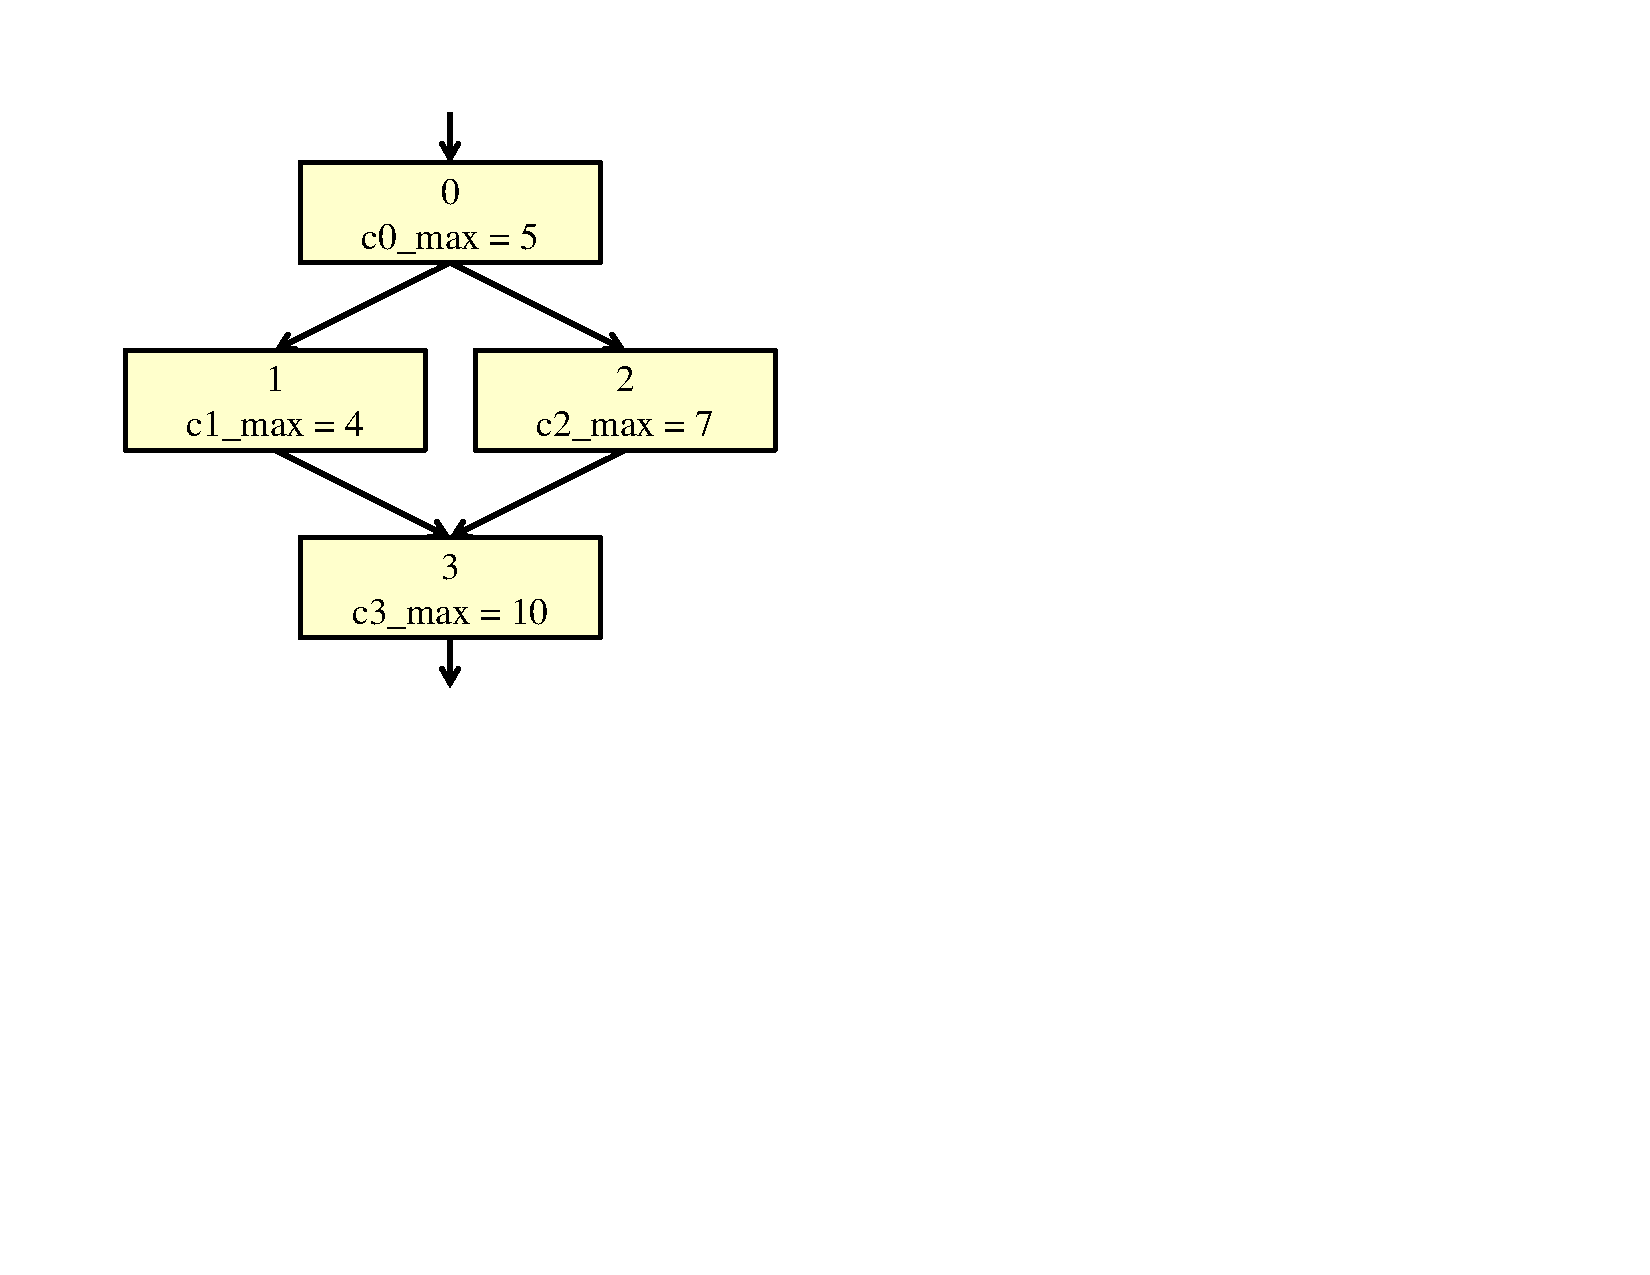
\includegraphics[width=3.5in]{monitoring_wcet/figs/cfg.pdf}
    \caption{Control flow graph of a main task.}
    \label{fig:monitoring_wcet.example.cfg}
  \end{center}
\end{figure}

The control flow graph for an example main task is shown in
Figure~\ref{fig:monitoring_wcet.example.cfg}. We assume that the worst-case
execution time for each node has already been calculated using previous
methods. These execution times are labeled as {\tt cB\_max} in the figure.

In this example, let us assume that the monitoring technique requires loads and
stores to be forwarded, as in the case of an uninitialized memory check (UMC).
The monitoring task requires 5 cycles to handle a load and 7 cycles to handle a
store. Thus, the maximum execution time of the monitoring task, $t_{M, max}$,
is 7 cycles.

Because of the simplicity of the example, we assume that the FIFO only holds
one entry ($n_F = 1$). Thus, $l_{max} = n_F \cdot t_{M, max} = 7$.

\subsection{Creating the MFG}

The first step is to create the monitoring flow graph. For each node in the
CFG, the code represented by that node is analyzed. After any forwarded
instruction, in this case any load or store instructions, an edge is created,
dividing a node into two nodes in the monitoring flow graph.  For example, the
assembly-level code for node 1 in the CFG is shown below.
\lstset{numbers=left, 
  firstnumber=1, 
  xleftmargin=2em, 
  numbersep=1em, 
  basicstyle=\ttfamily, 
  title=node 1, 
  } 
\begin{lstlisting}[frame=tb]
  add $t0, $t1, $t2
  add $t3, $t4, $t5
  lw  $t4, 0($t3)
  add $t0, $t0, $t4
\end{lstlisting}
Since the third instruction is a load instruction, node 1 must be split into
two nodes in the MFG. The first node represents the first three instructions
and the second node represents the last instruction. 

% MFG
\begin{figure}
  \begin{center}
    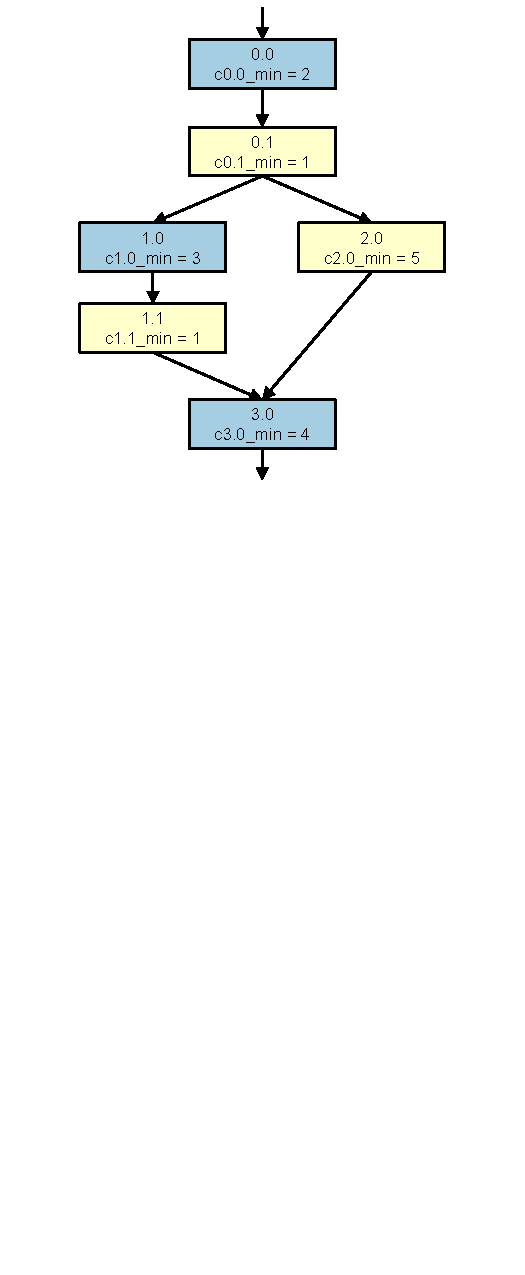
\includegraphics[width=3.5in]{monitoring_wcet/figs/mfg.pdf}
    \caption{Monitoring flow graph of the main task. Blue (dark) nodes indicate
    ones with a forwarded instruction at the end. Yellow (light) nodes indicate
    ones without a forwarded instruction.}
    \label{fig:monitoring_wcet.example.mfg}
  \end{center}
\end{figure}

The resulting MFG is shown in Figure~\ref{fig:monitoring_wcet.example.mfg}.
Nodes that are blue (dark) include a forwarded instruction, which is located at
the end of the node. Nodes that are yellow (light) do not include a forwarded
instruction. The nodes in the graph are labeled with minimum ({\tt cB\_min})
rather than maximum execution times. It can be seen that node 1 from the CFG
corresponds to nodes 1.0 and 1.1 in the MFG. In this example, nodes in the CFG
were only transformed into at most two nodes in the MFG.  However, in general,
a CFG node will be transformed into a number of nodes in the MFG equal to the
number of forwarded instructions plus one.

\subsection{Calculating the Monitoring Load}
Once the MFG is constructed, a set of MILP constraints is generated for each
node. This process can be automated, but for this example we will construct the
constraints for one node by hand. Specifically we will consider node 3.0 in the
MFG. We will also calculate, by hand, the MILP solution for the node using some
assumed values for variables associated with other nodes. Note that all
variables are assumed to be non-negative unless otherwise specified.

{\bf Calculating input monitoring load:}
First, we will determine the worst-case input monitoring load for node 3.0,
$li_{3.0}$.  One set of constraints lower bounds the monitoring load by all
possible incoming monitoring loads.
\begin{align*}
  li_{3.0} \geq& lo_{1.1} \\
  li_{3.0} \geq& lo_{2.0} 
\end{align*}
Then, a set of constraints upper bounds this input monitoring load.
\begin{align*}
  li_{3.0} - 1000 \delta_{1.1} \leq& lo_{1.1} \\
  li_{3.0} - 1000 \delta_{2.0} \leq& lo_{2.0} \\
  \delta_{1.1} + \delta_{2.0} =& 1
\end{align*}
Here, the value 1000 is chosen arbitrarily but is known to be greater than
$|lo_{2.0} - lo_{1.1}|$.  A different value could have been chosen as long as
this condition was true.  $\delta_{1.1}$ and $\delta_{2.0}$ are binary
variables which can only assume values of $0$ or $1$.  To see how these
constraints work, suppose that $li_{2.0} = 7$ and $li_{1.1} = 4$. The
constraints are then evaluated as
\begin{align*}
  li_{3.0} \geq& 4 \\
  li_{3.0} \geq& 7 \\
  li_{3.0} - 1000 \delta_{1.1} \leq& 4 \\
  li_{3.0} - 1000 \delta_{2.0} \leq& 7 \\
  \delta_{1.1} + \delta_{2.0} =& 1
\end{align*}
The first pair of constraints ensures that $li_{3.0} \geq 7$. This means that
for the third constraint to hold, $\delta_{1.1} = 1$. If $\delta_{1.1} = 1$,
then by the last constraint, $\delta_{2.0} = 0$. Plugging this value into the
fourth constraint gives $li_{3.0} \leq 7$. Thus, the only possible solution is
$li_{3.0} = 7$ which is the maximum of $lo_{1.1}$ and $lo_{2.0}$.

{\bf Calculating output monitoring load:}
In order to determine the output monitoring load for node 3.0, we must first
calculate the change in monitoring node, $\Delta l_{3.0}$. Since there is a
forwarded instruction in node 3.0,
\begin{align*}
  \Delta l_{3.0} =& t_{M, max} - c_{3.0, min} \\
  =& 7 - 4 = 3
\end{align*}
We first create a variable, $lo'_{3.0}$ to represent the unbounded output
monitoring load.
\begin{align*}
  lo'_{3.0} =& li_{3.0} + \Delta l_{3.0}, \text{ } lo'_{3.0} \in (-\infty, \infty)
\end{align*}
Using the example input monitoring load previously calculated of $li_{3.0} =
7$, this unbounded output monitoring load is $lo'_{3.0} = 7 + 3 = 10$.  Then,
the following set of constraints determines the bounded output monitoring load,
$lo_{3.0}$.
\begin{subequations}
\begin{align}
  -1000\lambda_3 + 7\lambda_5 + 1000\lambda_6 =& 10 \label{eq:monitoring_wcet.lo1}\\ 
  \lambda_3 + \lambda_4 + \lambda_5 + \lambda_6 =& 1 \label{eq:monitoring_wcet.lo2}\\
  2 \delta_3 + \lambda_5 + \lambda_6 \leq& 2 \label{eq:monitoring_wcet.lo3}\\
  2 \delta_4 + \lambda_3 + \lambda_6 \leq& 2 \label{eq:monitoring_wcet.lo4}\\
  2 \delta_5 + \lambda_3 + \lambda_4 \leq& 2 \label{eq:monitoring_wcet.lo5}\\
  \delta_3 + \delta_4 + \delta_5 = 1 \label{eq:monitoring_wcet.lo6}\\
  7\lambda_5 + 7\lambda_6 =& lo_{3.0} \label{eq:monitoring_wcet.lo7}
\end{align}
\end{subequations}
The -1000 and 1000 values were chosen arbitrarily and only require that
$lo'_{3.0}$ to fall between them. $\delta_3$, $\delta_4$, and $\delta_5$ are
binary variables. By Constraint~\ref{eq:monitoring_wcet.lo2}, it can be seen
that all $\lambda_i$ are less than or equal to 1. Thus, in order for
Constraint~\ref{eq:monitoring_wcet.lo1} to hold, $\lambda_6 >  0$. Since
$\lambda_6 > 0$, Constraints~\ref{eq:monitoring_wcet.lo3} and
\ref{eq:monitoring_wcet.lo4} force $\delta_3$ and $\delta_4$ to both be zero.
From this, by Constraint~\ref{eq:monitoring_wcet.lo6}, $\delta_5 = 1$. Then, by
Constraint~\ref{eq:monitoring_wcet.lo5}, $\lambda_3$ and $\lambda_4$ are both
forced to be zero. If we now go back to the first two constraints, they are
reduced to
\begin{align*}
  7\lambda_5 + 1000\lambda_6 =& 10\\
  \lambda_5 + \lambda_6 =& 1 \\
\end{align*}
Solving this system of equations gives the solution $(\lambda_5, \lambda_6) =
(0.997, 0.003)$. Plugging these values into Constraint~\ref{eq:monitoring_wcet.lo7},
\begin{align*}
  lo_{3.0} =& 7\lambda_5 + 7\lambda_6 \\
  =& 7\cdot 0.997 + 7\cdot 0.003 \\
  =& 7
\end{align*}
Thus, the output monitoring load is indeed bound by the maximum monitoring load
of 7. Although this may seem to be a complicated series of calculations to
determine this obvious result, this set of constraints is required in order for
the piecewise linear, and thus non-linear, bounding function to be expressed in
an MILP problem.

{\bf Calculating the monitoring stall cycles:} The one remaining value that
needs to be determined for node 3.0 is the monitoring stall cycles. Based on
our previous calculations, the worst-case input monitoring load ($li_{3.0}$) is
7, the change in monitoring load ($\Delta l_{3.0}$) is 3, and the maximum
monitoring load ($l_{max}$) is 7. Thus, we expect the worst-case monitoring
stall cycles to be $(7+3)-7 = 3$. To handle this as an MILP problem, first the
unbounded monitoring stall cycles, $s'$, is calculated.
\begin{align*}
  s'_{3.0} =& li_{3.0} + \Delta l_{3.0} - l_{max}, \text{ } s'_{3.0} \in (-\infty, \infty) \\
  =& 7 + 3 - 7 = 3
\end{align*}
In this case, since $s'_{3.0}$ is positive, we expect $s_{3.0} = s'_{3.0}$. The
MILP problem determines $s_{3.0}$ using the following set of constraints.
\begin{subequations}
\begin{align}
  -1000\lambda_0 + 1000\lambda_2 =& 3 \label{eq:monitoring_wcet.s1}\\
  \lambda_0 + \lambda_1 + \lambda_2 =& 1 \label{eq:monitoring_wcet.s2}\\
  \delta_1 + \lambda_2 \leq& 1 \label{eq:monitoring_wcet.s3}\\
  \delta_2 + \lambda_0 \leq& 1 \label{eq:monitoring_wcet.s4}\\
  \delta_1 + \delta_2 =& 1 \label{eq:monitoring_wcet.s5}\\
  1000\lambda_2 =& s_{3.0} \label{eq:monitoring_wcet.s6}
\end{align}
\end{subequations}
The -1000 and 1000 values are chosen arbitrarily, only requiring that
$s'_{3.0}$ is between them. From Constraint~\ref{eq:monitoring_wcet.s1},
$\lambda_2$ must be positive. Since $\delta_i$ are binary variables,
Constraint~\ref{eq:monitoring_wcet.s3} then implies that $\delta_1 = 0$.
Constraints~\ref{eq:monitoring_wcet.s4} and \ref{eq:monitoring_wcet.s5} then
force $\delta_2 = 1$ and $\lambda_0 = 0$. The first two constraints then reduce
to
\begin{align*}
  1000\lambda_2 =& 3\\
  \lambda_1 + \lambda_2 =& 1 
\end{align*}
Solving this system of equations leads to $(\lambda_1, \lambda_2) = (0.997,
0.003)$ and thus calculating $s_{3.0}$ using
Constraint~\ref{eq:monitoring_wcet.s6}:
\begin{align*}
  s_{3.0} =& 1000 \lambda_2 \\
  =& 1000 \cdot 0.003 = 3
\end{align*}
This is the value for $s$ that we expected. If $s'$ had instead been negative,
then $\delta_1$ would be forced to 1 and $\lambda_2$ would be forced to 0. From
the last constraint, it can be seen that if $\lambda_2$ is 0, then $s$ is also
0.

\subsection{MILP Optimization}

In the previous subsection, the monitoring loads for one node were calculated
in detail. However, note that the output monitoring load for each node with an
edge pointing to node 3.0 was assumed to be a certain value. In an actual MILP
problem, these would be variables that are also being solved for. Solving for
these inter-related variables and determining the global maximum number of
cycles stalled due to monitoring is impractical to do by hand.  While the
amount of calculations may seem excessive for these simple examples, the
ability to formulate the problem in MILP is essential in order to solve large
problems. Given an MILP formulation, existing solvers \cite{lpsolve, cplex} can
be used to obtain the worst-case stall cycles.

